+\chapter{Desarrollo de la solución}\label{CAP6}
    
    
    En este capitulo se explica la solución adoptada para validar la cinemática y dinámica de un robot delta. Para ello implementan 3 herramientas a este trabajo: ROS, RVIZ y ADAMS. 
    
    \begin{center}
        \smartdiagram[bubble diagram]{Solucion,ROS,RVIZ,ADAMS}
    \end{center}

    Diagrama de flujo (nodo principal + rviz + adams) en grandes explicaicons

    SIN PSEUDOCODIGO!!!! SOLO NOMBRAR EL NOMBRE DEL ARCHIVO
    Diagrama de flujo nodo principal path linear st ( sin nomine de funciones solo los pasos)

        \newpage

\section{Software ROS}

    Robot Operating Processing es una herramienta que sirve para ordenar y dividir en tareas especificas un robot complejo simplificando a los ingenieros la creación de estos. Estas tareas se representan en nodos, funciones y subfunciones que son escritos en lenguaje de programación python. En esta sección, estos algoritmos son explicados brevemente como una función con entradas y salidas definidas como se muestra en la ilustración \ref{f:Cap6_funtion_1} y explicados detalladamente en pseudocódigos como se puede visualizar en el algoritmo \ref{algo:cap6_1}. Los algoritmos se dividen en una función principal y en sus subfunciones.
    
        % Define block styles
        \tikzstyle{block1} = [rectangle, draw=blue,fill=blue!20, text width=10em, text centered, minimum height=7em, minimum width=2.5em , text=black]
        \tikzstyle{block2} = [rectangle, draw=black!50,fill=black!20, text width=10em, text centered, minimum height=4em, minimum width=2.5em ]
        \tikzstyle{line} = [draw, -latex']
         \begin{center}
         \begin{figure}[htb]
             \begin{tikzpicture}[node distance = 5cm, auto]
                % Place nodes
                \node [block1] (funcion) {\textbf{Objetivo\\del\\Algoritmo\\(Funcion)}};
                \node [block2, left of=funcion] (input) {\textbf{Entradas\\(Input)}};
                \node [block2, right of=funcion] (ouput) {\textbf{Salidas\\(Output)}};
                % Draw edges
                \path [line] (funcion) -- node {}(ouput);
                \path [line] (input) -- node { }(funcion);
            \end{tikzpicture}
                \caption{Fotografía de un paraguas}
                \label{f:Cap6_funtion_1}
         \end{figure}
         \end{center}

     \begin{algorithm}[H]
            \caption{Nombre del Algoritmo} 
            \label{algo:cap6_1}
            \SetKwInput{KwInput}{Input}                % Set the Input
            \SetKwInput{KwOutput}{Output}              % set the Output
            \SetKwInput{KwObjetivo}{Objetivo}                % Set the Input
            \SetKwInput{Kwfile}{Nombre archivo}                % Set the Input
            
            \DontPrintSemicolon
              \KwObjetivo {Explicación breve del objetivo principal del algoritmo}
              \Kwfile{Nombre del archivo donde se encuentra el código del algoritmo}
              \KwInput{$Entradas$}
              \KwOutput{$Salidas$}
              
                % Set Function Names
              \SetKwFunction{FSum}{$nombre.funcion.principal$}
              \SetKwFunction{FSub}{$nombre.subfunciones$}
            
              \tcc{FUNCION PRINCIPAL}
              \SetKwProg{Fn}{}{:}{}
              \Fn{\FSum{$Input$}}{
              \tcc{Algoritmo funcion principal*}
               \KwRet $Output$\;
              }
          \tcc{SUBFUNCIONES}
          \SetKwProg{Fn}{}{:}{}
          \Fn{\FSub{$Input$, {\phi}_i}}{
              \tcc{Algoritmo de subfunciones*}
                \KwRet$Output$\;
          }
    \end{algorithm}
    
    
        \newpage


    Las tareas realizadas en ROS son principalmente los conceptos teóricos del capitulo \ref{CAP4}:

\tikzset{
  basic/.style  = {draw, text width=2cm, drop shadow, font=\sffamily, rectangle},
  root/.style   = {basic, rounded corners=2pt, thin, align=center, fill=white},
  level-2/.style = {basic, rounded corners=6pt, thin,align=center, fill=white, text width=3cm},
  level-3/.style = {basic, thin, align=center, fill=white, text width=2.2cm}
}

\begin{center}
        \begin{figure}[H]
            \begin{tikzpicture}[
                  level 1/.style={sibling distance=10em, level distance=7em},
                %   {edge from parent fork down},
                  edge from parent/.style={->,solid,black,thick,sloped,draw}, 
                  edge from parent path={(\tikzparentnode.south) -- (\tikzchildnode.north)},
                  >=latex, node distance=1.9cm, edge from parent fork down]
    
                % root of the the initial tree, level 1
                \node[root] {\textbf{Algoritmos ROS}}
                % The first level, as children of the initial tree
                  child {node[level-2] (c1) {\textbf{Metodologia\\  A}}}
                  child {node[level-2] (c2) {\textbf{Metodologia\\  B}}}
                  child {node[level-2] (c3) {\textbf{Espacio \\ de\\  Trabajo}}}
                  child {node[level-2] (c4) {\textbf{Trayectoria}}};
                
                % The second level, relatively positioned nodes
                \begin{scope}[every node/.style={level-3}]
                    \node [below of = c1, xshift=10pt] (c11) {Cinematica Directa};
                    \node [below of = c11] (c12) {Cinematica Inversa};
                    \node [below of = c12] (c13) {Jacobiano};
                    \node [below of = c13] (c14) {Cinematica\\de\\Aceleracion};
                    \node [below of = c14] (c15) {Dinamica Inversa};
    
                    \node [below of = c2, xshift=10pt] (c21) {Cinematica Directa};
                    \node [below of = c21] (c22) {Cinematica Inversa};
                    \node [below of = c22] (c23) {Jacobiano};
                    \node [below of = c23] (c24) {Cinematica\\de\\Aceleracion};
                    \node [below of = c24] (c25) {Dinamica Inversa};
    
                \end{scope}
                
                % lines from each level 1 node to every one of its "children"
                \foreach \value in {1,2,3,4,5}
                  \draw[->] (c1.195) |- (c1\value.west);
                
                \foreach \value in {1,2,3,4,5}
                  \draw[->] (c2.195) |- (c2\value.west);
                
            \end{tikzpicture}
            
                \caption{This is a simple Taxonomy}
                \label{fig:my_label}
        \end{figure}
 \end{center}
   
    \newpage

    \subsection{Metodología A}
    
    Las siguientes ilustraciones (\ref{f:Cap6_funtion_2} a la \ref{f:Cap6_funtion_6}) representan de forma visual los algoritmos, tareas o funciones planteadas en esta sección con respecto a la  metodología A del capitulo \ref{CAP4}, de igual forma que en la ilustración \ref{f:Cap6_funtion_1}. Las entradas y las salidas de cada función son escritas con las misma nomenclatura de cada sección con que fue inspirado el algoritmo respectivamente. Es notorio recalcar que cada algoritmo es obtenido de diferentes referencias bibliográficas, por lo que los sistemas de referencia y el orden numérico de los ángulos de los actuadores son diferentes. Por ende, las entradas y las salidas en cada algoritmo son transformadas del sistema global al sistema de referencia local y viceversa.     
    

            \hspace{1cm}


    % Define block styles
    \tikzstyle{block1} = [rectangle, draw=blue,fill=blue!20, text width=10em, text centered, minimum height=3em, minimum width=2.5em , text=black]
    \tikzstyle{block2} = [rectangle, draw=black!50,fill=black!20, text width=10em, text centered, minimum height=3em, minimum width=2.5em ]
    \tikzstyle{line} = [draw, -latex']

    \begin{figure}[h]
        \centering
        \begin{subfigure}
                \centering
                 \begin{tikzpicture}[node distance = 5cm, auto]
                    % Place nodes
                    \node [block1] (funcion) {\textbf{Cinemática Directa\\ Sección (\ref{ma_cd})}};
                    \node [block2, left of=funcion] (input) {\textbf{$\theta_1,\theta_2,\theta_3$}};
                    \node [block2, right of=funcion] (ouput) {\textbf{$E_0(x_0,y_0,z_0)$}};
                    % Draw edges
                    \path [line] (funcion) -- node {}(ouput);
                    \path [line] (input) -- node { }(funcion);
                \end{tikzpicture}
                    \caption{Fotografía de un paraguas}
                    \label{f:Cap6_funtion_2}
        \end{subfigure}
        
        \hspace{1cm}

        \begin{subfigure}
                \centering
                 \begin{tikzpicture}[node distance = 5cm, auto]
                    % Place nodes
                    \node [block1] (funcion) {\textbf{Cinemática Inversa\\ Sección (\ref{ma_ci})}};
                    \node [block2, left of=funcion] (input) {\textbf{$E_0(x_0,y_0,z_0)$}};
                    \node [block2, right of=funcion] (ouput) {\textbf{$\theta_1,\theta_2,\theta_3$}};
                    % Draw edges
                    \path [line] (funcion) -- node {}(ouput);
                    \path [line] (input) -- node { }(funcion);
                \end{tikzpicture}
                    \caption{Fotografía de un paraguas}
                    \label{f:Cap6_funtion_3}
        \end{subfigure}
        
                \hspace{1cm}

        \begin{subfigure}
                \centering
                 \begin{tikzpicture}[node distance = 5cm, auto]
                    % Place nodes
                    \node [block1] (funcion) {\textbf{Jacobiano\\ Sección (\ref{ma_cvel})}};
                    \node [block2, left of=funcion] (input) {\textbf{$P_x,P_y,P_z,{\theta }_{11},{\theta }_{12},{\theta }_{13}$}};
                    \node [block2, right of=funcion] (ouput) {\textbf{$ J,J_{\theta }, J_{x },$\\$\theta _{31},\theta _{32},\theta _{33},$\\$\theta _{21},\theta _{22},\theta _{23}$}};
                    % Draw edges
                    \path [line] (funcion) -- node {}(ouput);
                    \path [line] (input) -- node { }(funcion);
                \end{tikzpicture}
                    \caption{Fotografía de un paraguas}
                    \label{f:Cap6_funtion_4}
         \end{subfigure}
         
         
                 \hspace{1cm}

        \begin{subfigure}
                \centering
                 \begin{tikzpicture}[node distance = 5cm, auto]
                    % Place nodes
                    \node [block1] (funcion) {\textbf{Cinemática Aceleracion\\ Sección (\ref{})}};
                    \node [block2, left of=funcion] (input) {\textbf{Entradas}};
                    \node [block2, right of=funcion] (ouput) {\textbf{Salidas}};
                    % Draw edges
                    \path [line] (funcion) -- node {}(ouput);
                    \path [line] (input) -- node { }(funcion);
                \end{tikzpicture}
                    \caption{Fotografía de un paraguas}
                    \label{f:Cap6_funtion_5}
         \end{subfigure}
         
                 \hspace{1cm}

        \begin{subfigure}
                \centering
                 \begin{tikzpicture}[node distance = 5cm, auto]
                    % Place nodes
                    \node [block1] (funcion) {\textbf{Dinamica Inversa\\ Sección (\ref{})}};
                    \node [block2, left of=funcion] (input) {\textbf{Entradas}};
                    \node [block2, right of=funcion] (ouput) {\textbf{Salidas}};
                    % Draw edges
                    \path [line] (funcion) -- node {}(ouput);
                    \path [line] (input) -- node { }(funcion);
                \end{tikzpicture}
                    \caption{Fotografía de un paraguas}
                    \label{f:Cap6_funtion_6}
         \end{subfigure}
                \hspace{1cm}
    \end{figure}








    \newpage

 \subsubsection{Cinemática directa}
    \begin{algorithm}[H]
        \caption{Cinemática Directa Metodología A} 
        \label{algo:cap6_2}
        \SetKwInput{KwInput}{Input}                % Set the Input
        \SetKwInput{KwOutput}{Output}              % set the Output
        \SetKwInput{KwObjetivo}{Objetivo}                % Set the Input
        \SetKwInput{Kwfile}{Nombre archivo}                % Set the Input
        
        \DontPrintSemicolon
          \KwObjetivo {Hallar la posición del efector final del robot delta dada una configuración articular}
          \Kwfile{$delta.kinematics.t1m.adams.py$}
          \KwInput{$\theta_1,\theta_2,\theta_3$}
          \KwOutput{$E_0(x_0,y_0,z_0)$}
          
          % Set Function Names{\theta }_1,{\theta }_2,{\theta }_3
          \SetKwFunction{FSub}{forward}
           \SetKwProg{Fn}{}{:}{}
        
          \tcc{FUNCION PRINCIPAL}
            \Fn{\FSub{${\theta }_1$,${\theta }_2$,${\theta }_3$}}{
                \tcc{Cambiar angulos al orden del sistema de referencia local}
                \tcc{Calcular Centros de esferas (Ecuaciones tabla [\ref{tab:cap4_tabla_3}])}
                $(x_1,y_1,z_1)$=${J^'}_1\left(0,\left[-\frac{f-e}{2\sqrt{3}}-r_f{\mathrm{cos} \left({\theta }_1\right)\ }\right],-r_f{\mathrm{sin}\mathrm{n} \left({\theta }_1\right)\ }\right)$\;
                $(x_2,y_2,z_2)$=${J^'}_2(\left[\frac{f-e}{2\sqrt{3}}+r_f{\mathrm{cos} \left({\theta }_2\right)\ }\right]\mathrm{cos}\mathrm{}(30{}^\circ ),\left[\frac{f-e}{2\sqrt{3}}+r_f{\mathrm{cos} \left({\theta }_2\right)\ }\right]\mathrm{sin}\mathrm{}(30{}^\circ ),-r_f{\mathrm{sin} \left({\theta }_2\right)\ })$\;
                $(x_3,y_3,z_3)$=${J^'}_3(-\left[\frac{f-e}{2\sqrt{3}}+r_f{\mathrm{cos} \left({\theta }_3\right)\ }\right]\mathrm{cos}\mathrm{}(30{}^\circ ),\left[\frac{f-e}{2\sqrt{3}}+r_f{\mathrm{cos} \left({\theta }_3\right)\ }\right]\mathrm{sin}\mathrm{}(30{}^\circ ),-r_f{\mathrm{sin} \left({\theta }_3\right)\ })$\;
                \tcc{Calcular intersección de las 3 esferaS (Ecuaciones de la \ref{eq:cap4_eq_3} a la \ref{eq:cap4_eq_13})}
                $d= \left(y_2- y_1\right)x_3-\left(y_3-y_1\right)x_2- \left(y_2-y_3\right)x_1$\;
                $w_1={x_1}^2+{y_1}^2 +{z_1}^2$\;
                $w_2={x_2}^2+{y_2}^2 +{z_2}^2$\;
                $w_3={x_3}^2+{y_3}^2 +{z_3}^2$\;
                $a_1=\frac{\left(z_2-z_1\right)\left(y_3-y_1\right)-\left(z_3-z_1\right)\left(y_2-y_1\right)}{d}$\;
                $b_1=\left(\frac{1}{2*(-d)}\right)*\left(\left(w_2 - w_1\right)\left(y_3-y_1\right)-\left(w_3 - w_1\right)\left(y_2-y_1\right)\right)$\;
                $a_2=\frac{-1}{d}*\left[\left(z_2-z_1\right)x_3-(z_3-z_1)x_2+(z_3-z_2)x_1\right]$\;
                $b_2=\frac{1}{2d}*[\left(w_2-w_1\right)x_3-\left(w_3-w_1\right)x_2+\left(w_3-w_2)x_1\right]$\;
                $A = {a_1}^2+{a_2}^2+1$\;
                $B = 2(a_1(b_1-x_1)+a_2(b_2-y_1)-z_1)$\;
                $C=  ({(b_1-x_1)}^2+{(b_2-y_1)}^2+{z_1}^2- {r_e}^2)$\;
                $E_0(x_0,y_0,z_0) =  \left(a_1z+\ b_1,a_2z+\ b_2,\frac{-B-\ \sqrt{\left(B^2\right)-\left(4AC\right)}}{2A}\right)$\;
                           \KwRet  $(x_0,y_0,z_0)$\;
                }
    \end{algorithm}
    
    \newpage
 
 \subsubsection{Cinemática inversa}
     \begin{algorithm}[H]
            \caption{Cinemática Inversa Metodología A} 
            \SetKwInput{KwInput}{Input}                % Set the Input
            \SetKwInput{KwOutput}{Output}              % set the Output
            \SetKwInput{KwObjetivo}{Objetivo}                % Set the Input
            \SetKwInput{Kwfile}{Nombre archivo}                % Set the Input
            
            \DontPrintSemicolon
              \KwObjetivo {Hallar la posición de los actuadores en el espacio articular dada la posición del centroide del efector final}
              \Kwfile{$delta.kinematics.t1m.adams.py$}
              \KwInput{$E_0(x_0,y_0,z_0)$}
              \KwOutput{${\theta }_1$,${\theta }_2$,${\theta }_3$}
              
                % Set Function Names
              \SetKwFunction{FSum}{inverse}
              \SetKwFunction{FSub}{$angle.yz$}
            
              \tcc{FUNCION PRINCIPAL}
              \SetKwProg{Fn}{}{:}{}
              \Fn{\FSum{$x_0,y_0,z_0$}}{
              \tcc{Rotación del sistema de referencia Local en $0^{\circ}$}
                ${x}_{0 ^{\circ}}=x_0$\;
                ${y}_{0 ^{\circ}}=y_0$\;
                ${z}_{0 ^{\circ}}=z_0$\;
              \tcc{Rotación del sistema de referencia Local en $120^{\circ}$}
                ${x}_{120 ^{\circ}}=x_0*cos120+y_0*sin120$\;
                ${y}_{120 ^{\circ}}=y_0*cos120-x_0*sin120$\;
                ${z}_{120 ^{\circ}}=z_0$\;
              \tcc{Rotación del sistema de referencia Local en $240^{\circ}$}
                ${x}_{240 ^{\circ}}=x_0*cos120-y_0*sin120$\;
                ${y}_{240 ^{\circ}}=y_0*cos120+x_0*sin120$\;
                ${z}_{240 ^{\circ}}=z_0$\;
                
              \tcc{Calcular angulos de los actuadores}
              \tcc{Cambiar orden de ángulos al sistema Referencia Global}
                 ${\theta }_2=angle.yz({x}_{0 ^{\circ}} , {y}_{0 ^{\circ}} , {z}_{0 ^{\circ}},0 ^{\circ})$\;    
                 ${\theta }_3=angle.yz({x}_{120 ^{\circ}},{y}_{120 ^{\circ}},{z}_{120 ^{\circ}},120 ^{\circ})$\;
                 ${\theta }_1=angle.yz({x}_{240 ^{\circ}},{y}_{240 ^{\circ}},{z}_{240 ^{\circ}},240 ^{\circ})$\;
            
               \KwRet $[{\theta }_1,{\theta }_2,{\theta }_3]$\;
              }
    \end{algorithm}
    
\newpage

    \begin{algorithm}
          \ContinuedFloat
          \caption{Cinemática Inversa Metodología A (Continuacion...)}
          \tcc{SUBFUNCIONES}
          \SetKwProg{Fn}{}{:}{}
          \Fn{\FSub{${x}_{{ \phi }_i} , {y}_{{ \phi }_i} , {z}_{{ \phi }_i}$, { \phi }_i}}{
               \tcc{Actuador $F_{i}$ en el plano $Y'Z'$ (sistema de referencia Local rotado en ${ \phi }_i$)}
                $y_{1}= y_{F_{i}} = -\frac{f}{2\sqrt[]{3}}$\;
                $z_{1}=z_{F_{i}}=0$\;        
               \tcc{ Proyección de la Junta Esférica $E_{i}$ en el plano $Y'Z'$(sistema de referencia Local rotado en ${ \phi }_i$)}    
                $y_{2}= y_{E'_{i}} = {y}_{{ \phi }_i}-\frac{e}{2\sqrt[]{3}}$\;
                $z_{2}=z_{E'_{i}}={z}_{{ \phi }_i} $\;
                \tcc{Junta Esférica $J_{i}$ de la cadena cinemática i en posición ${ \phi }_i$}
                $a=\frac{{x}_{{ \phi }_i}^{2}+y_{2}^{2}+{z}_{{ \phi }_i}^{2}+r_{f}^{2}- r_{e}^{2}~-y_{1}^{2}}{2{z}_{{ \phi }_i}}$\;
                $b=\frac{ \left( y_{1}-y_{2} \right) }{z_{2}}$\;
                $x_{J_{i}}=0$\;
                $y_{J_{i}}=$ $\frac{(y_{1}-ab )-\sqrt{ -(a+by_{1}) ^{2}+ (b^{2}+1)r_{f}^{2}}}{b^{2}+1}$\;
                $z_{J_{i}}=a+b*y_{J_{i}}$\;
                \tcc{ Calculo del Angulo ${\theta }_i$ de la cadena cinemática i en posición ${ \phi }_i$}
                ${\theta }_i=\arctan( ~\frac{z_{J_{i}}}{y_{F_{i}}-y_{J_{i}}})$\;
                \KwRet${\theta }_i$\;
          }
    \end{algorithm}

 
\newpage
  
        
    \subsubsection{Jacobiano}
            
        \begin{algorithm}[H]
            \caption{Jacobiano Metodología A} 
            \SetKwInput{KwInput}{Input}                % Set the Input
            \SetKwInput{KwOutput}{Output}              % set the Output
            \SetKwInput{KwObjetivo}{Objetivo}                % Set the Input
            \SetKwInput{Kwfile}{Nombre archivo}                % Set the Input
            
              \DontPrintSemicolon
              \KwObjetivo {Hallar la matriz jacobiana}
              \Kwfile{$jacobian.tm1.adams.py$}
              \KwInput{$P_x,P_y,P_z,{\theta }_{11},{\theta }_{12},{\theta }_{13}$}
              \KwOutput{ $J_{\theta }, J_{x },\theta _{31},\theta _{32},\theta _{33},\theta _{21},\theta _{22},\theta _{23}, J$}
               
                % Set Function Names,
              \SetKwFunction{FSum}{jacobian.total}
              \SetKwFunction{FSub}{calculo.theta3i}
            
              \tcc{FUNCION PRINCIPAL}
              \SetKwProg{Fn}{}{:}{}
              \Fn{\FSum{$P_x$,$P_y$,$P_z$,${\theta }_{11}$,${\theta }_{12}$,${\theta }_{13}$}}{
                  \tcc{Cambiar ángulos y punto P al sistema Referencia Local}
                   $({\phi}_{0 ^{\circ}},{\phi}_{120 ^{\circ}},{\phi}_{240 ^{\circ}})=(0,120,240)$\;
                  \tcc{Calcular angulo $\theta _{3i}$ y $\theta _{2i}$}
                  $\theta _{31}=calculo.theta3i(P_x,P_y, {\phi}_{0 ^{\circ}})$\;
                  $\theta _{32}=calculo.theta3i(P_x,P_y, {\phi}_{120 ^{\circ}})$\;
                  $\theta _{33}=calculo.theta3i(P_x,P_y, {\phi}_{240 ^{\circ}})$\;
                  $\theta _{21}=calculo.theta2i(P_x,P_y,P_z,{\theta }_{31}, {\phi}_{0 ^{\circ}})$\;
                  $\theta _{22}=calculo.theta2i(P_x,P_y,P_z,{\theta }_{32}, {\phi}_{120 ^{\circ}})$\;
                  $\theta _{23}=calculo.theta2i(P_x,P_y,P_z,{\theta }_{33}, {\phi}_{240 ^{\circ}})$\;
                  \tcc{Calcular Matriz $J_{x}$ }
                  $ J_{1x}=calculo.jix($\theta _{11},\theta _{21},\theta _{31},${ \phi }_{0 ^{\circ}})$\;
                  $ J_{2x}=calculo.jix($\theta _{12},\theta _{22},\theta _{32},${ \phi }_{120 ^{\circ}})$\;
                  $ J_{3x}=calculo.jix($\theta _{13},\theta _{23},\theta _{33},${ \phi }_{240 ^{\circ}})$\;
                  $ J_{1y}=calculo.jiy($\theta _{11},\theta _{21},\theta _{31},${ \phi }_{0 ^{\circ}})$\;
                  $ J_{2y}=calculo.jiy($\theta _{12},\theta _{22},\theta _{32},${ \phi }_{120 ^{\circ}})$\;
                  $ J_{3y}=calculo.jiy($\theta _{13},\theta _{23},\theta _{33},${ \phi }_{240 ^{\circ}})$\; 
                   $ J_{1z}=calculo.jiz($\theta _{11},\theta _{21},\theta _{31},${ \phi }_{0 ^{\circ}})$\;
                  $ J_{2z}=calculo.jiz($\theta _{12},\theta _{22},\theta _{32},${ \phi }_{120 ^{\circ}})$\;
                  $ J_{3z}=calculo.jiz($\theta _{13},\theta _{23},\theta _{33},${ \phi }_{240 ^{\circ}})$\; 
                  $ J_{x}=[J_{1x},J_{1y},J_{1z};J_{2x},J_{2y},J_{2z};J_{3x},J_{3y},J_{3z}]$\;
                  \tcc{Calcular Matriz $J_{ \theta }$ }
                    $J_{1 \theta }=calculo.jthetai(\theta_{21}$,$\theta _{31}$,$\phi_{0 ^{\circ}})$\;
                    $J_{2 \theta }=calculo.jthetai(\theta_{22}$,$\theta _{32}$,$\phi_{120 ^{\circ}})$\;
                    $J_{3 \theta }=calculo.jthetai(\theta_{23}$,$\theta _{33}$,$\phi_{240 ^{\circ}})$\;
                    $J_{ \theta }=[J_{1 \theta },0,0;0,J_{2 \theta },0;0,0,J_{3 \theta }]$\;  
                \tcc{Calcular Matriz $J$ }
                    $J=J_{x}^{-1}J_{ \theta } $\;
                \tcc{Cambiar al sistema Referencia Global al operar}
                  \KwRet $[J_{\theta }, J_{x},\theta _{31},\theta _{32},\theta _{33},\theta _{21},\theta _{22},\theta _{23}, J]$\;}
        \end{algorithm}
        
\newpage

\begin{algorithm}
          \ContinuedFloat
          \caption{Jacobiano Metodología A (Continuacion...)}
          \tcc{SUBFUNCIONES}
          
          \tcc{Calcular angulo ${\theta }_{3i}$}  
          \SetKwProg{Fn}{}{:}{}
          \Fn{\FSub{$P_x$,$P_y$ ,$\phi_i$}}{
            $c_{yi}= (-P_x)*(sin({ \phi }_i))+(P_y)*(cos({ \phi }_i))$\;    
            $\theta _{3i}= \cos ^{-1}\frac{c_{yi}}{b}$\;    
                \KwRet${\theta }_{3i}$\;   } 
        
          \tcc{Calcular angulo ${\theta }_{2i}$}
          \SetKwProg{Fn}{}{:}{}
          \SetKwFunction{FSub}{calculo.theta2i}
          \Fn{\FSub{$P_x$,$P_y$,$P_z$,${\theta }_{3i}$,$\phi_i$}}{
                      	$c_{xi}=(P_x)*(cos({ \phi }_i))+(P_y)*(sin({ \phi }_i))+ h-r$\; 
            	$c_{yi}= (-P_x)*(sin({ \phi }_i))+(P_y)*(cos({ \phi }_i))$\; 
        	    $c_{zi}=P_z$\; 
        
                $\theta _{2i}=\cos ^{-1} \left( \frac{c_{xi}^{2}+c_{yi}^{2}+c_{zi}^{2}-a^{2}-b^{2}~}{2ab sin~ \theta _{3i}} \right)$\;        
                \KwRet${\theta }_{2i}$\;  }
                
                
           \tcc{Calcular componentes Matriz $J_x$}
           \SetKwFunction{FSub}{calculo.jix}
           \SetKwProg{Fn}{}{:}{}
           \Fn{\FSub{$\theta _{1i}$,$\theta _{2i}$,$\theta _{3i}$, $\phi_i$}}{
            $ J_{ix}=\cos  \left(  \theta _{1i}+ \theta _{2i} \right) sin~ \theta _{3i}\cos  \phi _{i}-cos  \theta _{3i}\sin  \phi _{i}~ $\;    
            \KwRet$J_{ix}$\;  }
                
                
          \SetKwFunction{FSub}{calculo.jiy}
           \SetKwProg{Fn}{}{:}{}
          \Fn{\FSub{$\theta _{1i}$,$\theta _{2i}$,$\theta _{3i}$,$\phi_i$}}{
            $J_{iy}=\cos  \left(  \theta _{1i}+ \theta _{2i} \right) sin~ \theta _{3i}\sin  \phi _{i}+ cos  \theta _{3i}\cos  \phi _{i}~$\;    
            \KwRet$J_{iy}$\;  }   
                    
            
           \SetKwFunction{FSub}{calculo.jiz}
           \SetKwProg{Fn}{}{:}{}
          \Fn{\FSub{$\theta _{1i}$,$\theta _{2i}$,$\theta _{3i}$,$\phi_i$}}{
            $ J_{iz}=sin \left(  \theta _{1i}+ \theta _{2i} \right) sin~ \theta _{3i}~ $\;    
            \KwRet$J_{iz}$\;} 
            
          \tcc{Calcular componentes Matriz $J_{\theta }$}
          \SetKwFunction{FSub}{calculo.jthetai}
          \Fn{\FSub{$\theta_{2i}$,$\theta _{3i}$,$\phi_i$}}{
                $J_{i \theta }=a~\sin  \theta _{2i}~sin~ \theta _{3i}$\; 
                \KwRet$J_{i \theta }$\;   }
\end{algorithm}


        \newpage
        \subsubsection{Cinematica de Aceleracion}



        \newpage
        \subsubsection{Dinámica Inversa}
        
        
        
        
        
        
        
        
        
        
        
        
        
        
        
        
        
        
        
        
        \newpage

        
    \subsection{Metodología B}
    
       Al igual que la sección anterior, se presentan en las ilustraciones \ref{f:Cap6_funtion_7} a la \ref{f:Cap6_funtion_11} las tareas con respecto a la  metodología B del capitulo \ref{CAP4}. 
    
            \hspace{1cm}


    % Define block styles
    \tikzstyle{block1} = [rectangle, draw=blue,fill=blue!20, text width=10em, text centered, minimum height=3em, minimum width=2.5em , text=black]
    \tikzstyle{block2} = [rectangle, draw=black!50,fill=black!20, text width=10em, text centered, minimum height=3em, minimum width=2.5em ]
    \tikzstyle{line} = [draw, -latex']

    \begin{figure}[h]
        \centering
        \begin{subfigure}
                \centering
                 \begin{tikzpicture}[node distance = 5cm, auto]
                    % Place nodes
                    \node [block1] (funcion) {\textbf{Cinemática Directa\\ Sección (\ref{mb_cd})}};
                    \node [block2, left of=funcion] (input) {\textbf{$\theta_1,\theta_2,\theta_3$}};
                    \node [block2, right of=funcion] (ouput) {\textbf{$P_0(P_{0x},P_{0y},P_{0z})$}};
                    % Draw edges
                    \path [line] (funcion) -- node {}(ouput);
                    \path [line] (input) -- node { }(funcion);
                \end{tikzpicture}
                    \caption{Fotografía de un paraguas}
                    \label{f:Cap6_funtion_7}
        \end{subfigure}
        
        \hspace{1cm}

        \begin{subfigure}
                \centering
                 \begin{tikzpicture}[node distance = 5cm, auto]
                    % Place nodes
                    \node [block1] (funcion) {\textbf{Cinemática Inversa\\ Sección (\ref{mb_ci})}};
                    \node [block2, left of=funcion] (input) {\textbf{$P_0(P_{0x},P_{0y},P_{0z})$}};
                    \node [block2, right of=funcion] (ouput) {\textbf{$\theta_1,\theta_2,\theta_3$}};
                    % Draw edges
                    \path [line] (funcion) -- node {}(ouput);
                    \path [line] (input) -- node { }(funcion);
                \end{tikzpicture}
                    \caption{Fotografía de un paraguas}
                    \label{f:Cap6_funtion_8}
        \end{subfigure}
        
                \hspace{1cm}

        \begin{subfigure}
                \centering
                 \begin{tikzpicture}[node distance = 5cm, auto]
                    % Place nodes
                    \node [block1] (funcion) {\textbf{Jacobiano\\ Sección (\ref{mb_cvel})}};
                    \node [block2, left of=funcion] (input) {\textbf{$P_{0x},P_{0y},P_{0z},{\theta }_{1},{\theta }_{2},{\theta }_{3}$}};
                    \node [block2, right of=funcion] (ouput) {\textbf{$-J_{1 }, J_{2}, J$}};
                    % Draw edges
                    \path [line] (funcion) -- node {}(ouput);
                    \path [line] (input) -- node { }(funcion);
                \end{tikzpicture}
                    \caption{Fotografía de un paraguas}
                    \label{f:Cap6_funtion_9}
         \end{subfigure}
         
         
                 \hspace{1cm}

        \begin{subfigure}
                \centering
                 \begin{tikzpicture}[node distance = 5cm, auto]
                    % Place nodes
                    \node [block1] (funcion) {\textbf{Cinemática Aceleracion\\ Sección (\ref{})}};
                    \node [block2, left of=funcion] (input) {\textbf{Entradas}};
                    \node [block2, right of=funcion] (ouput) {\textbf{Salidas}};
                    % Draw edges
                    \path [line] (funcion) -- node {}(ouput);
                    \path [line] (input) -- node { }(funcion);
                \end{tikzpicture}
                    \caption{Fotografía de un paraguas}
                    \label{f:Cap6_funtion_10}
         \end{subfigure}
         
                 \hspace{1cm}

        \begin{subfigure}
                \centering
                 \begin{tikzpicture}[node distance = 5cm, auto]
                    % Place nodes
                    \node [block1] (funcion) {\textbf{Dinamica Inversa\\ Sección (\ref{})}};
                    \node [block2, left of=funcion] (input) {\textbf{Entradas}};
                    \node [block2, right of=funcion] (ouput) {\textbf{Salidas}};
                    % Draw edges
                    \path [line] (funcion) -- node {}(ouput);
                    \path [line] (input) -- node { }(funcion);
                \end{tikzpicture}
                    \caption{Fotografía de un paraguas}
                    \label{f:Cap6_funtion_11}
         \end{subfigure}
                \hspace{1cm}
    \end{figure}
    
            \newpage

    
        \subsubsection{Cinemática directa}
        
\begin{algorithm}[H]
    \caption{Cinemática Directa Metodología B} 
    \SetKwInput{KwInput}{Input}                % Set the Input
    \SetKwInput{KwOutput}{Output}              % set the Output
    \SetKwInput{KwObjetivo}{Objetivo}                % Set the Input
    \SetKwInput{Kwfile}{Nombre archivo}                % Set the Input
    
    \DontPrintSemicolon
      \KwObjetivo {Hallar la posición del efector final del robot delta dada una configuración articular}
      \Kwfile{$delta.kinematics.Paderborn.tm1.adams$}
      \KwInput{$\theta_1,\theta_2,\theta_3$}
      \KwOutput{$P_0(P_{0x},P_{0y},P_{0z})$}
      
      % Set Function Names{\theta }_1,{\theta }_2,{\theta }_3
      \SetKwFunction{FSub}{forward.Paderborn}
       \SetKwProg{Fn}{}{:}{}
    
      \tcc{FUNCION PRINCIPAL}
        \Fn{\FSub{${\theta }_1$,${\theta }_2$,${\theta }_3$}}{
            \tcc{Calcular Centros de esferas (Ecuaciones (\ref{eq:cap4_MB_3}),(\ref{eq:cap4_MB_4}),(\ref{eq:cap4_MB_5}))}
            \tcc{Ordenar angulos segun sistema de referencia Local}
            
            $(x_1,y_1,z_1)$=$\overrightarrow{J'_{2}} \left [  0,-\frac{(f-e)}{2\sqrt{3}}-L_{A}cos(\theta_2),-L_{A}sin(\theta_2)\right]$\;
            
            $(x_2,y_2,z_2)$=$\overrightarrow{J'_{3}} \left [\left( \frac{(f-e)}{2\sqrt{3}}+{L}_{A}cos(\theta_3)\right) cos(30^\circ), \left(\frac{(f-e)}{2\sqrt{3}} + {L}_{A}cos(\theta_3)\right) sin(30^\circ), -L_{A}sin(\theta_3)\right]$\;
            
            $(x_3,y_3,z_3)$=$\overrightarrow{J'_{1}} \left [\left( \frac{(f-e)}{2\sqrt{3}}+{L}_{A}cos(\theta_1)\right) cos(30^\circ), \left(\frac{(f-e)}{2\sqrt{3}} + {L}_{A}cos(\theta_1)\right) sin(30^\circ), -L_{A}sin(\theta_1)\right]$\;
            
            \tcc{Calcular intersección de las 3 esferaS (Ecuaciones de la \ref{eq:cap4_eq_3} a la \ref{eq:cap4_eq_13})}
            $d= \left(y_2- y_1\right)x_3-\left(y_3-y_1\right)x_2- \left(y_2-y_3\right)x_1$\;
            $w_1={x_1}^2+{y_1}^2 +{z_1}^2$\;
            $w_2={x_2}^2+{y_2}^2 +{z_2}^2$\;
            $w_3={x_3}^2+{y_3}^2 +{z_3}^2$\;
            $a_1=\frac{\left(z_2-z_1\right)\left(y_3-y_1\right)-\left(z_3-z_1\right)\left(y_2-y_1\right)}{d}$\;
            $b_1=\left(\frac{1}{2*(-d)}\right)*\left(\left(w_2 - w_1\right)\left(y_3-y_1\right)-\left(w_3 - w_1\right)\left(y_2-y_1\right)\right)$\;
            $a_2=\frac{-1}{d}*\left[\left(z_2-z_1\right)x_3-(z_3-z_1)x_2+(z_3-z_2)x_1\right]$\;
            $b_2=\frac{1}{2d}*[\left(w_2-w_1\right)x_3-\left(w_3-w_1\right)x_2+\left(w_3-w_2)x_1\right]$\;
            $A = {a_1}^2+{a_2}^2+1$\;
            $B = 2(a_1(b_1-x_1)+a_2(b_2-y_1)-z_1)$\;
            $C=  ({(b_1-x_1)}^2+{(b_2-y_1)}^2+{z_1}^2- {r_e}^2)$\;
            $P_0(P_{0x},P_{0y},P_{0z}) =  \left(a_1z+\ b_1,a_2z+\ b_2,\frac{-B-\ \sqrt{\left(B^2\right)-\left(4AC\right)}}{2A}\right)$\;
                       \KwRet  $(P_{0x},P_{0y},P_{0z})$\;
            }
\end{algorithm}

\newpage        
 
        
     
        
        \newpage

\subsubsection{Cinemática inversa}
        
    \begin{algorithm}[H]
            \caption{Cinemática Inversa Metodología B} 
            \SetKwInput{KwInput}{Input}                % Set the Input
            \SetKwInput{KwOutput}{Output}              % set the Output
            \SetKwInput{KwObjetivo}{Objetivo}                % Set the Input
            \SetKwInput{Kwfile}{Nombre archivo}                % Set the Input
            
            \DontPrintSemicolon
              \KwObjetivo {Hallar la posición de los actuadores en el espacio articular dada la posición del centroide del efector final}
              \Kwfile{$delta.kinematics.Paderborn.tm1.adams$}
              \KwInput{$P_0(P_{0x},P_{0y},P_{0z})$}
              \KwOutput{${\theta }_1$,${\theta }_2$,${\theta }_3$}
              
                % Set Function Names
              \SetKwFunction{FSum}{inverse.Paderborn}
              \SetKwFunction{FSub}{$angle.yz.Paderborn$}
            
              \tcc{FUNCION PRINCIPAL}
              \SetKwProg{Fn}{}{:}{}
              \Fn{\FSum{$P_{0x},P_{0y},P_{0z}$}}{
              \tcc{Rotación del sistema de referencia Local en $0^{\circ}$}
                ${x}_{0 ^{\circ}}=P_{0x}$\;
                ${y}_{0 ^{\circ}}=P_{0y}$\;
                ${z}_{0 ^{\circ}}=P_{0z}$\;
              \tcc{Rotación del sistema de referencia Local en $120^{\circ}$}
                ${x}_{120 ^{\circ}}=P_{0x}*cos120+P_{0y}*sin120$\;
                ${y}_{120 ^{\circ}}=P_{0y}*cos120-P_{0x}*sin120$\;
                ${z}_{120 ^{\circ}}=P_{0z}$\;
              \tcc{Rotación del sistema de referencia Local en $240^{\circ}$}
                ${x}_{240 ^{\circ}}=P_{0x}*cos120-P_{0y}*sin120$\;
                ${y}_{240 ^{\circ}}=P_{0y}*cos120+P_{0x}*sin120$\;
                ${z}_{240 ^{\circ}}=P_{0z}$\;
                
              \tcc{Calcular angulos de los actuadores}
              \tcc{Cambiar orden de ángulos al sistema Referencia Global}
                 ${\theta }_2=angle.yz.Paderborn({x}_{0 ^{\circ}} , {y}_{0 ^{\circ}} , {z}_{0 ^{\circ}},0 ^{\circ})$\;    
                 ${\theta }_3=angle.yz.Paderborn({x}_{120 ^{\circ}},{y}_{120 ^{\circ}},{z}_{120 ^{\circ}},120 ^{\circ})$\;
                 ${\theta }_1=angle.yz.Paderborn({x}_{240 ^{\circ}},{y}_{240 ^{\circ}},{z}_{240 ^{\circ}},240 ^{\circ})$\;
            
               \KwRet $[{\theta }_1,{\theta }_2,{\theta }_3]$\;
              }
    \end{algorithm}
    
    \clearpage   
        
\begin{algorithm}
      \ContinuedFloat
      \caption{Cinemática Inversa Metodología B (Continuacion...)}
      \tcc{SUBFUNCIONES}
      \SetKwProg{Fn}{}{:}{}
      \Fn{\FSub{${x}_{{ \varphi }_i} , {y}_{{ \varphi }_i} , {z}_{{ \varphi }_i}$, { \varphi }_i}}{
           \tcc{Actuador $F_{i}$ en el plano $Y'Z'$ (sistema de referencia Local rotado en ${ \varphi }_i$)}
            $y_{1}= y_{F_{i}} = -\frac{f}{2\sqrt[]{3}}$\;
            $z_{1}=z_{F_{i}}=0$\;        
           \tcc{ Proyección de la Junta Esférica $P_{0}$ en el plano $Y'Z'$(sistema de referencia Local rotado en ${ \varphi }_i$)}    
            $y_{2}= y_{P'_{0}} = {y}_{{ \varphi }_i}-\frac{e}{2\sqrt[]{3}}$\;
            $z_{2}=z_{P'_{0}}={z}_{{ \varphi }_i} $\;
            \tcc{Junta Esférica $J_{i}$ de la cadena cinemática i en posición ${ \varphi }_i$}
            $a=\frac{{x}_{{ \varphi }_i}^{2}+y_{2}^{2}+{z}_{{ \varphi }_i}^{2}+R_{A}^{2}- R_{B}^{2}~-y_{1}^{2}}{2{z}_{{ \varphi }_i}}$\;
            $b=\frac{ \left( y_{1}-y_{2} \right) }{z_{2}}$\;
            $x_{J_{i}}=0$\;
            $y_{J_{i}}=$ $\frac{(y_{1}-ab )-\sqrt{- (a+by_{1}) ^{2}+ (b^{2}+1)R_{A}^{2}}}{b^{2}+1}$\;
            $z_{J_{i}}=a+b*y_{J_{i}}$\;
            \tcc{ Calculo del Angulo ${\theta }_i$ de la cadena cinemática i en posición ${ \varphi }_i$}
            ${\theta }_i=\arctan( ~\frac{z_{J_{i}}}{y_{F_{i}}-y_{J_{i}}})$\;
            \KwRet${\theta }_i$\;
      }
\end{algorithm}
    
        \newpage

 \subsubsection{Jacobiano}
     
         \begin{algorithm}[H]
            \caption{Jacobiano Metodología B} 
            \SetKwInput{KwInput}{Input}                % Set the Input
            \SetKwInput{KwOutput}{Output}              % set the Output
            \SetKwInput{KwObjetivo}{Objetivo}                % Set the Input
            \SetKwInput{Kwfile}{Nombre archivo}                % Set the Input
            
            \DontPrintSemicolon
              \KwObjetivo {Hallar la matriz jacobiana}
              \Kwfile{$jacobian.Paderborn.tm1.v2.adams.py$}
              \KwInput{$P_{0x},P_{0y},P_{0z},{\theta }_{1},{\theta }_{2},{\theta }_{3}$}
              \KwOutput{ $-J_{1 }, J_{2}, J$}
               
                % Set Function Names,
              \SetKwFunction{FSum}{jacobian.calculo.Paderborn}

              \tcc{FUNCION PRINCIPAL}
              \SetKwProg{Fn}{}{:}{}
              \Fn{\FSum{$P_x$,$P_y$,$P_z$,${\theta }_{11}$,${\theta }_{12}$,${\theta }_{13}$}}{
              \tcc{Cambiar ángulos y punto P al sistema Referencia Local}
              \tcc{Posición actuadores $\varphi$ respecto a ejes $YX$ S.ref Local}
              $({\phi}_{0 ^{\circ}},${\phi}_{120 ^{\circ}},${\phi}_{240 ^{\circ}})=(0,120,240)$\;

              \tcc{Calcular  $\overrightarrow{s_{i}}$ Transpose  }
              $\overrightarrow{s_{1}}^T={si(P_{0x},P_{0y},P_{0z},{\theta }_{1},\varphi_{0 ^{\circ}})}^T$\;
              $\overrightarrow{s_{2}}^T={si(P_{0x},P_{0y},P_{0z},{\theta }_{2},\varphi_{120 ^{\circ}})}^T$\;
              $\overrightarrow{s_{3}}^T={si(P_{0x},P_{0y},P_{0z},{\theta }_{3},\varphi_{240 ^{\circ}})}^T$\;
              \tcc{Calcular $\overrightarrow{b_{i}}$  }
              $\overrightarrow{b_{1}}={bi({\theta }_{1},\varphi_{0 ^{\circ}})}$\;
              $\overrightarrow{b_{2}}={bi({\theta }_{2},\varphi_{120 ^{\circ}})}$\;
              $\overrightarrow{b_{3}}={bi({\theta }_{3},\varphi_{240 ^{\circ}})}$\;
              
              \tcc{Calcular componentes $J_{1}$ }
              $J_{1}$=\left.    
              {\begin{bmatrix}
                 $\overrightarrow{s_{1}}^T(0)$ & $\overrightarrow{s_{1}}^T(1)$ & $\overrightarrow{s_{1}}^T(2)$\\
                $\overrightarrow{s_{2}}^T(0)$ & $\overrightarrow{s_{2}}^T(1)$ & $\overrightarrow{s_{2}}^T(2)$\\
                $\overrightarrow{s_{3}}^T(0)$ & $\overrightarrow{s_{3}}^T(1)$ & $\overrightarrow{s_{3}}^T(2)$ 
            \end{bmatrix}}^{-1}
            \right.

              \tcc{Calcular $J_{2}$ }
              $J_{2}$=\left.    
              \begin{bmatrix}
                 $\overrightarrow{s_{1}}^T \cdot \overrightarrow{b_{1}} $ & $0$ & $0$\\
                $0$ & $\overrightarrow{s_{2}}^T \cdot \overrightarrow{b_{2}}$ & $0$\\
                $0$ & $0$ & $\overrightarrow{s_{3}}^T \cdot \overrightarrow{b_{3}}$
            \end{bmatrix}
            \right.

              \tcc{Calcular $J$ ecuacion (\ref{eq:cap4_MB_14}) }
                $J=-J_{1}J_{2}$\;
                
               
            \tcc{Cambiar al sistema Referencia Global al operar $J$}
              \KwRet $[-J_{1},J_{2},J]$   }
        \end{algorithm}
 

\begin{algorithm}
          \ContinuedFloat
          \caption{Jacobiano Metodología B (Continuacion...)}
          \tcc{SUBFUNCIONES}
          
          \tcc{Calcular $\overrightarrow{s_{i}}$ }
          \SetKwProg{Fn}{}{:}{}
          \SetKwFunction{FSub}{si}
          \Fn{\FSub{$P_{0x}$,$P_{0y}$,$P_{0z}$,${\theta }_{i}$,$\varphi_i$}}{
                \tcc{Vector efector final }
                $\overrightarrow{P_{0}}=
                \left.          
                \begin{bmatrix}
                P_{0x} \\
                P_{0y} \\
                P_{0z}
            \end{bmatrix}  \right.$\;
                \tcc{Matriz de rotacion respecto a ángulo 
               $\varphi_i$ }
            $R_{i}^{R}=matri.rot(\varphi_i)$\;
            \tcc{Vector posición actuador i respecto a sistema referencia local }
            $R={R}_{A}-{R}_{B}$\;
            $ \overrightarrow{F_{i}}=R_{i}^{R} 
                \left.          
                \begin{bmatrix}
               R \\
                0 \\
                0
            \end{bmatrix}  \right.$\;
            \tcc{Vector brazo i respecto a sistema referencia local }
             $\overrightarrow{\xi_{F_{i}J_{i}}}=R_{i}^{R}
              \left.          
                \begin{bmatrix}
               L_{A} cos(\theta_i) \\
                0 \\
                -L_{A} sin(\theta_i)
            \end{bmatrix}  \right.$\;
            \tcc{calculo $\overrightarrow{s_{i}}$ ecuacion (\ref{eq:cap4_MB_12})}
            $ \overrightarrow{s_{i}} & = \overrightarrow{P_{0}}- \left(\overrightarrow{F_{i}}+\overrightarrow{\xi_{F_{i}J_{i}}} \right)$\;
            \KwRet$\overrightarrow{s_{i}}$\;  }
                
          \tcc{Calcular $\overrightarrow{b_{i}}$ }
          \SetKwProg{Fn}{}{:}{}
          \SetKwFunction{FSub}{bi}
          \Fn{\FSub{${\theta }_{i}$,$\varphi_i$}}{
                \tcc{Matriz de rotacion respecto a ángulo 
               $\varphi_i$ }
            $R_{i}^{R}=matri.rot(\varphi_i)$\;
            \tcc{calculo $\overrightarrow{b_{i}}$ ecuacion (\ref{eq:cap4_MB_15}) }
            $ \overrightarrow{b_{i}} =  R_{i}^{R}      \begin{bmatrix}
                L_{A} sin(\theta_i) \\
                0\\
                L_{A} cos(\theta_i) 
            \end{bmatrix}$\;
            \KwRet$\overrightarrow{b_{i}}$\;  }
        
          \tcc{Calcular Matriz de rotacion $R_{i}^{R}$ ecuacion (\ref{eq:cap4_MB_13})}
          \SetKwProg{Fn}{}{:}{}
          \SetKwFunction{FSub}{matri.rot}
          \Fn{\FSub{$\varphi_i$}}{
            $ R_{i}^{R} =
        \begin{bmatrix}
                cos(\varphi_i)&-sin(\varphi_i)&0 \\
                sin(\varphi_i)&cos(\varphi_i)&0 \\
                0&0&1
            \end{bmatrix}$\;
            \KwRet$R_{i}^{R}$\;  }
\end{algorithm}

        \newpage

\subsubsection{Cinematica de Aceleracion}

            \newpage


\subsubsection{Dinámica Inversa}
        \newpage

        
    \subsection{Espacio de Trabajo}
     Encontrar el espacio de trabajo de un robot delta significa calcular todas las posiciones posibles y viables del efector final. El siguiente diagrama de flujo representa una de las muchas soluciones que existen, donde las dimensiones del robot y los parámetros de las restricciones son valores preestablecidos. Es importante recalcar que la nomenclatura en esta sección es la misma que se implementa para determinar el jacobiano del robot delta de la sección \ref{ma_jac}.  
    
             \begin{figure}[htb]
                \centering
                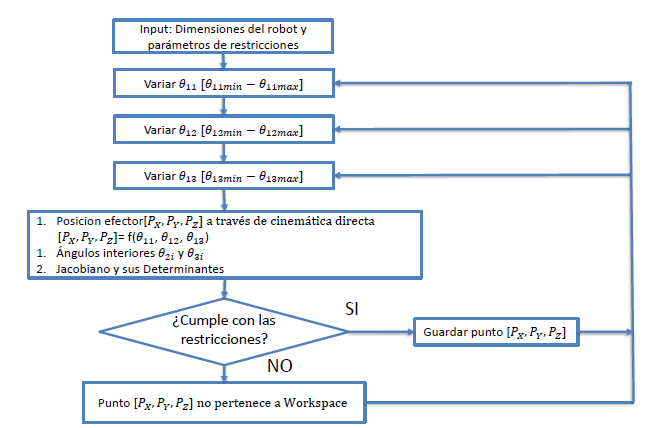
\includegraphics[width=1\linewidth]{Main/Chapter6/Images6/cap6_ws_2.png}
                \caption{Fotografía de un paraguas}
                \label{f:Cap6_ws_2}
            \end{figure}  

    CAMBIARDIAGRAMA La idea principal de la solución propuesta es calcular un grupo significativo de configuraciones $(P_x,P_y,P_z)$ posibles del efector final en base a sus dimensiones y evaluar si cumplen con restricciones impuestas. Se obtienen las configuraciones cartesianas del efector $(P_x,P_y,P_z)$  utilizando la cinemática directa y variando los angulos $\theta_{11}$,$\theta_{12}$,$\theta_{13}$ en los rangos $[\theta_{11min}-\theta_{11max}]$, $[\theta_{12min}-\theta_{12max}]$, $[\theta_{13min}-\theta_{13max}]$ respectivamente. Todos estos rangos se discretizan con un paso impuesto \(  \Delta  \theta _{1i} \). Si el punto  $(P_x,P_y,P_z)$ cumple con todas las restricciones, el punto pertenece al espacio de trabajo. Al contrario, si el punto no cumple con una o mas restricciones, este no pertenece al espacio de trabajo.

        \newpage

    Las restricciones son las mismas que las expuestas en la sección \ref{restriccionesWS}. El orden en que se verifican las restricciones se muestran en el siguiente diagrama de flujo:

             \begin{figure}[htb]
                \centering
                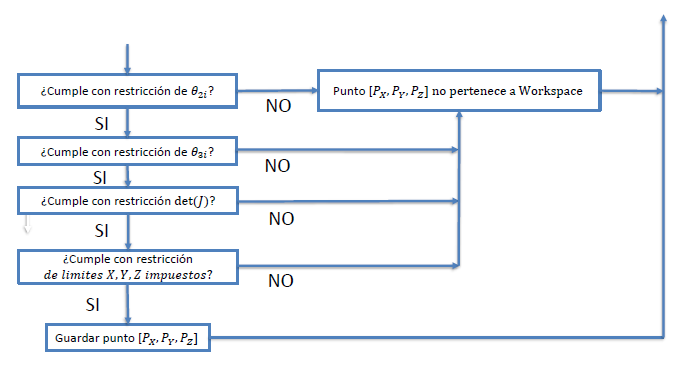
\includegraphics[width=1\linewidth]{Main/Chapter6/Images6/cap6_ws_3.png}
                \caption{Fotografía de un paraguas}
                \label{f:Cap6_ws_3}
            \end{figure}  


    Para calcular el espacio de trabajo se crea un nodo en ROS. La tarea especifica de este nodo es calcular, guardar y graficar los puntos $(P_x,P_y,P_z)$ del efector final que cumplen con las restricciones impuestas. 
    La representación gráfica del nodo se presenta en la ilustración \ref{f:Cap6_ws_1}: 
    
    
        % Define block styles
        \tikzstyle{block1} = [rectangle, draw=blue,fill=blue!20, text width=10em, text centered, minimum height=7em, minimum width=2.5em , text=black]
        \tikzstyle{block2} = [rectangle, draw=black!50,fill=black!20, text width=10em, text centered, minimum height=4em, minimum width=2.5em ]
        \tikzstyle{line} = [draw, -latex']
         \begin{center}
         \begin{figure}[htb]
             \begin{tikzpicture}[node distance = 5cm, auto]
                % Place nodes
                    \node [block1] (funcion) {\textbf{Espacio\\de\\Trabajo}};
                \node [block2, left of=funcion] (input) {\textbf{ $\Delta\theta _{1i}$\\$(Discretizacion$ $Espacio$ $Articular$$)$}};
                \node [block2, right of=funcion] (ouput) {\textbf{$\mathcal{W}_{(J_{x},J_{\theta})},\mathcal{W}_{J_{x}},\\\mathcal{W}_{J_{\theta}},\mathcal{W}_{(J_{x},J_{\theta},Limites)}$\\($Espacios$ $de$ $Trabajo$ $en$ $coordenadas$ $cartesianas$ $y$ $articular$)}};
                % Draw edges
                \path [line] (funcion) -- node {}(ouput);
                \path [line] (input) -- node { }(funcion);
            \end{tikzpicture}
                \caption{Fotografía de un paraguas}
                \label{f:Cap6_ws_1}
         \end{figure}
         \end{center}
         
        \vspace{-1cm}         
    
    En este nodo, las dimensiones del robot y las restricciones son establecidas antes de calcular el espacio de trabajo. La única entrada es el paso de la discretizacion de los rangos \(  \Delta  \theta _{1i} \). La cinematica directa y el jacobiano se calculan a partir del método A, específicamente los desarrollados en las secciones \ref{ma_cd} y \ref{ma_jac} respectivamente. Se emplea este método por la razón de que el jacobiano $J$ se puede bipartir en dos matrices $(J_{x}$  y  $J_{ \theta })$, donde cada una de ellas representa una singularidad especifica . Ademas, el metodo A tiene la ventaja que tiene las ecuaciones para determinar los ángulos interiores $\theta_{2i}$ y $\theta_{3i}$.
    
    \newpage
    
    El valor de los parámetros de las restricciones impuestas en este trabajo de grado se presentan y se explican en la tabla \ref{t:cap6_ws_1}: 
    
            \begingroup
            \renewcommand{\arraystretch}{1.5}
            \begin{table}[H]
            \centering
            \begin{tabular}{c m{7.5cm} c c}
               \hline
               \textbf{Restriccion}  & \textbf{Explicacion} & \textbf{Min}& \textbf{Max}\\
               \hline           \hline            
             $\theta_{1i}$ & Colisión entre los brazos y la base fija & $-90^{\circ}$ & $90^{\circ}$\\
            \hline
             $\Delta\theta _{1i}$ & Pasos de discretizacion de rangos $\theta_{1i}$ muy bajos implica costo computacional alto& $1^{\circ}$ & $90^{\circ}$ \\
            \hline
             $\theta _{2i}$ & Angulo debe ser menor a $180^{\circ}$ ya que en esa situación el brazo y antebrazo podrían ser colineales y producir singularidades. Ademas esta restriccion asegura que el calculo de la cinemática de posición sea la correcto ya que descarta una de las soluciones & $5^{\circ}$ & $175^{\circ}$ \\
            \hline
             $\theta _{3i}$ & Angulo respecto a la inclinación máxima de las rotulas por catalogo, generalmente son de $13^{\circ}$ & $75^{\circ}$ & $165^{\circ}$ \\
            \hline
             $J_{x}$ & Depende de la precisión o factor de seguridad subjetivo& $5*10^{-1}$ & $\inf$ \\
            \hline
             $J_{\theta}$ & Depende de la precisión o factor de seguridad subjetivo& $1*10^{-4}$ & $\inf$ \\
            \hline
             $X$ & Limite X de espacio de trabajo impuesto por el fabricante & $-100[mm]$ & $+100[mm]$ \\
            \hline            
             $Y$ & Limite Y de espacio de trabajo impuesto por el fabricante & $-100[mm]$ & $+100[mm]$ \\
            \hline   
             $Z$ & Limite Z de espacio de trabajo impuesto por el fabricante & $-100[mm]$ & $+100[mm]$ \\
            \hline   
            \end{tabular}
            \caption{Referencias del dibujo}
            \label{t:cap6_ws_1}
        \end{table}
        \endgroup     
        
         \begin{figure}[htb]
                \centering
                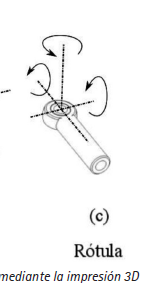
\includegraphics[width=0.1\linewidth]{Main/Chapter6/Images6/cap6_ws_4.png}
                \caption{Fotografía de un paraguas}
                \label{f:Cap6_ws_4}
            \end{figure}    
    
        \newpage

    El siguiente algoritmo presenta el pseudocódigo de la función dentro del nodo que determinar el espacio de trabajo:
    
\begin{algorithm}[H]
    \caption{Espacio de Trabajo} 
    \SetKwInput{KwInput}{Input}                % Set the Input
    \SetKwInput{KwOutput}{Output}              % set the Output
    \SetKwInput{KwObjetivo}{Objetivo}                % Set the Input
    \SetKwInput{Kwfile}{Nombre archivo}                % Set the Input
    
    \DontPrintSemicolon
      \KwObjetivo {Encontrar el espacio de trabajo del robot delta a partir de sus dimensiones y restricciones impuestas.}
      \Kwfile{$workspace.py$}
      \KwInput{ $\Delta\theta _{1i}$}
      \KwOutput{$[\mathcal{W}_{(J_{x},J_{\theta})},\mathcal{W}_{J_{x}},\mathcal{W}_{J_{\theta}},\mathcal{W}_{(J_{x},J_{\theta},Limites)}]$}
      
      % Set Function Names{\theta }_1,{\theta }_2,{\theta }_3
      \SetKwFunction{FSub}{espaciotrabajo}
       \SetKwProg{Fn}{}{:}{}
    
      \tcc{FUNCION PRINCIPAL}
        \Fn{\FSub{$\Delta\theta _{1i}$}}{
            \tcc{Barrido de angulos $\theta _{11}$ , $\theta _{12}$ y $\theta _{13}$ con incrementos de $\Delta\theta _{1i}$}
            \For{\theta _{11} \in [$\theta_{11min}$ - $\theta_{11max}]$;$\Delta\theta _{1i}$}    
                { 
                \For{\theta _{12} \in [$\theta_{12min}$ - $\theta_{12max}]$;$\Delta\theta _{1i}$}  
                    { 
                    \For{\theta _{13} \in [$\theta_{13min}$ - $\theta_{13max}]$;$\Delta\theta _{1i}$}    
                        { 
                        \tcc{Cinematica Directa}
                	     $(P_{x},P_{y},P_{z})=forward(\theta _{12},\theta _{13},\theta _{11})$\;
                        \tcc{Jacobiano}
                        $[J_{\theta},J_{x},\theta_{31},\theta_{32},\theta_{33},\theta_{21},\theta_{22},\theta_{23},J] = jacobian.total(P_{x},P_{y},P_{z},\theta_{11},\theta_{12},\theta_{13})   $\;
                        \tcc{Determinantes Jacobiano}
                        $\left|J_{\theta}\right|=det(J_{\theta})$\;
                        $\left|J_{x}\right|=det(J_{x})$\;
                         \tcc{Restricciones}
                          \If {$Restricciones$ $\theta_{2i}$} 
                              {
                                \If {$Restricciones$ $\theta_{3i}$} 
                                      {
                                      \If {$Restricciones$ $\left|J_{x}\right|$ o $\left|J_{\theta}\right|$} 
                                              {
                                              $\mathcal{W}_{(J_{x},J_{\theta})} =(P_{x},P_{y},P_{z},\theta_{11},\theta_{12},\theta_{13})$ \;
                                                  \If {$Restricciones$ $Limites XYZ$} 
                                                  { $\mathcal{W}_{(J_{x},J_{\theta},limites)}=(P_{x},P_{y},P_{z},\theta_{11},\theta_{12},\theta_{13})$ \;
                                                  }
                                              }
                                        \Else{$(P_{x},P_{y},P_{z})$ No pertenece al espacio de trabajo\;}
                                      \If {$Restricciones$ $\left|J_{x}\right|$} 
                                              {
                                               $\mathcal{W}_{J_{x}}=(P_{x},P_{y},P_{z},\theta_{11},\theta_{12},\theta_{13})$
                                              }
                                      \If {$Restricciones$ $\left|J_{\theta}\right|$} 
                                              {
                                               $\mathcal{W}_{J_{\theta}} =(P_{x},P_{y},P_{z},\theta_{11},\theta_{12},\theta_{13})$
                                              }
                                      
                                    }
                              }
                        }  
                    }           
                }
                       \KwRet  $[\mathcal{W}_{(J_{x},J_{\theta})},\mathcal{W}_{J_{x}},\mathcal{W}_{J_{\theta}},\mathcal{W}_{(J_{x},J_{\theta},Limites)}]$\;
            }
\end{algorithm}
    
    \newpage

    \subsection{Trayectoria}
    
    En esta seccion se explica el desarrollo para determinar la trayectoria en el espacio articular del robot delta, es decir, la trayectoria angular de los actuadores, a partir de una trayectoria lineal interpolada en el espacio cartesiano XYZ que recorre el efector final de un punto inicial $P_i$ a un punto final $P_f$ con restricciones de velocidad trapezoidal en dirección del camino geometrico.

        % Define block styles
        \tikzstyle{block1} = [rectangle, draw=blue,fill=blue!20, text width=10em, text centered, minimum height=5em, minimum width=2.5em , text=black]
        \tikzstyle{block2} = [rectangle, draw=black!50,fill=black!20, text width=10em, text centered, minimum height=4em, minimum width=2.5em ]
        \tikzstyle{line} = [draw, -latex']
         \begin{center}
         \begin{figure}[htb]
             \begin{tikzpicture}[node distance = 5cm, auto]
                % Place nodes
                    \node [block1] (funcion) {\textbf{Trayectoria}};
                \node [block2, left of=funcion] (input) {\textbf{$P_i$ $P_f$}};
                \node [block2, right of=funcion] (ouput) {\textbf{$Puntos$ $de$ $la$ \\ $Trayectoria$ \\$en$ $el$\\ $espacio$\\ $cartesiano$ $XYZ$}};
                % Draw edges
                \path [line] (funcion) -- node {}(ouput);
                \path [line] (input) -- node { }(funcion);
            \end{tikzpicture}
                \caption{Fotografía de un paraguas}
                \label{f:cap6_trayectory_1}
         \end{figure}
         \end{center}
         
        \vspace{-1cm}   

        
    Esta trayectoria se compone de un camino geométrico lineal en el espacio cartesiano XYZ se llaman 'punto a punto en linea recta' y la escala temporal es de 'Perfil de Movimiento Trapezoidal respecto a la Velocidad' o 'Linear segment with Parabolic Blends (LSPB)', visto en la sección \ref{cap4_tray}. 
    
    El perfil de movimiento trapezoidal visto en la sección \ref{Perfiles_de_movimiento_trapezoidal} se puede modificar para que las ecuaciones consideren el punto inicial y final especificando la velocidad máxima y la aceleracion maxima de la siguiente manera:
        \begin{equation}
        \Large
            q(t) = \left\lbrace
                \begin{array}{ll}
                q_0 + s\frac{a}{2}t^2&   0< t \leq \tau\\
                q_0 - s\frac{V^2}{2a}+sVt &  \tau< t \leq T- \tau\\
                q_1 + s \left( -\frac{aT^2}{2}+aTt-\frac{a}{2}t^2 \right) &  T- \tau< t \leq T\\
            \end{array}
            \right.
            \label{eq:cap6_tray_1}
        \end{equation}
    
    Donde:
    \begin{equation*}
       \text{$q_0$: $Punto$ $inicial$}
    \end{equation*}
    \begin{equation*}
       \text{$q_1$: $Punto$ $final$ }
    \end{equation*}
    \begin{equation*}
       \text{$V$: $velocidad$ $maxima$ $permitida$}
    \end{equation*}
    \begin{equation*}
       \text{$a$: $aceleracion$ $maxima$ $permitida$}
    \end{equation*}
    
    \newpage
    
    \begin{equation}
        \tau=\frac{V}{a}
    \label{eq:cap6_tray_4}
    \end{equation}
    \begin{equation}
        T=s\frac{q_1-q_0}{V}+\frac{V}{a}
    \label{eq:cap6_tray_5}
    \end{equation}
    \begin{equation}
        s=signo(q_1-q_0)
    \label{eq:cap6_tray_6}
    \end{equation}
    

     \begin{figure}[htb]
            \centering
            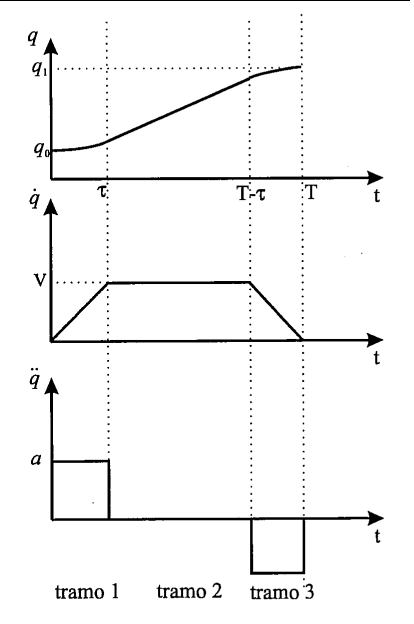
\includegraphics[width=0.7\linewidth]{Main/Chapter6/Images6/cap6_trayectory_2.png}
            \caption{Fotografía de un paraguas}
            \label{f:cap6_trayectory_2}
        \end{figure} 


    \newpage

    Para utilizar el perfil de velocidad trapezoidal en el camino geométrico lineal interpolado desde el punto inicial $P_i$ al punto final $P_f$ se aplican matrices de rotaciones. 
    
    
    \begin{enumerate}[1.]
        \item     Primero se traslada el sistema de referencia general $X_0Y_0Z_0$ al punto inicial $P_i$ generando un nuevo sistema de referencia $X_{trans}Y_{trans}Z_{trans}$ . 
        
        \item Luego se rota $X_{trans}Y_{trans}Z_{trans}$ sobre el eje $Z_{trans}$ en un angulo de $\theta_z$ generando un nuevo sistema de referencia $X_{rot_{\theta_z}}Y_{rot_{\theta_z}}Z_{rot_{\theta_z}}$. $\theta_z$  es el angulo interno entre el eje $X_{trans}$ y el vector   $\overrightarrow{$O_{X_{trans}Y_{trans}Z_{trans}}{P'}_f$}$ donde ${P'}_f$ es la  proyeccion de $P_f$ sobre el plano  $Y_{trans}Z_{trans}$.
        
        \item     Finalmente el marco de referencia $X_{rot_{\theta_z}}Y_{rot_{\theta_z}}Z_{rot_{\theta_z}}$ se rota sobre el eje  $Y_{rot_{\theta_z}}$ en un angulo de $\theta_y$ generando el ultimo sistema de referencia $X_{rot_{\theta_y}}Y_{rot_{\theta_y}}Z_{rot_{\theta_y}}$.
        $\theta_y$  es el angulo interno entre el eje $X_{rot_{\theta_z}}$ y el vector   $\overrightarrow{$O_{X_{rot_{\theta_z}}Y_{rot_{\theta_z}}Z_{rot_{\theta_z}}}{P''}_f$}$ donde ${P''}_f$ es el punto  ${P}_f$ con respecto al sistema de referencia  $X_{rot_{\theta_z}}Y_{rot_{\theta_z}}Z_{rot_{\theta_z}}$ .
         En el marco de referencia $X_{rot_{\theta_y}}Y_{rot_{\theta_y}}Z_{rot_{\theta_y}}$ se aplica el perfil de velocidad trapezoidal para que define la escala temporal de la trayectoria y la interpolación lineal en el espacio cartesiano del camino geométrico. 
    \end{enumerate}
    
     \begin{figure}[htb]
            \centering
            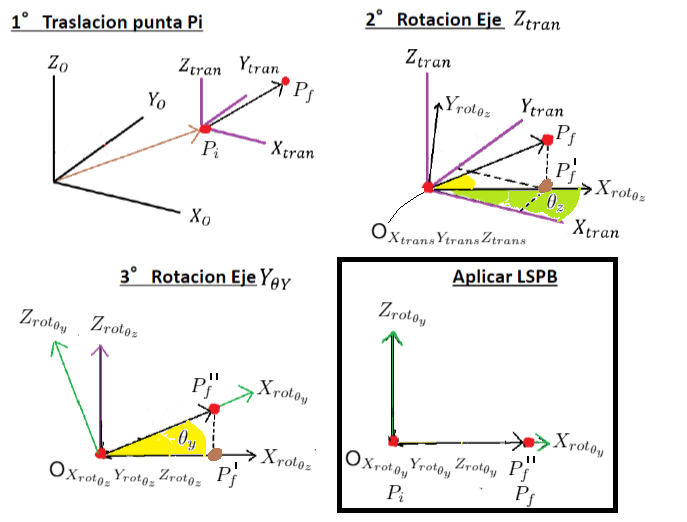
\includegraphics[width=1\linewidth]{Main/Chapter6/Images6/cap6_trayectory_3.png}
            \caption{Fotografía de un paraguas}
            \label{f:cap6_trayectory_3}
        \end{figure} 
        
    \newpage
        
    El diagrama de flujo para el desarrollo de la trayectoria se presenta en la ilustración \ref{f:cap6_trayectory_4}:
    
     \begin{figure}[htb]
            \centering
            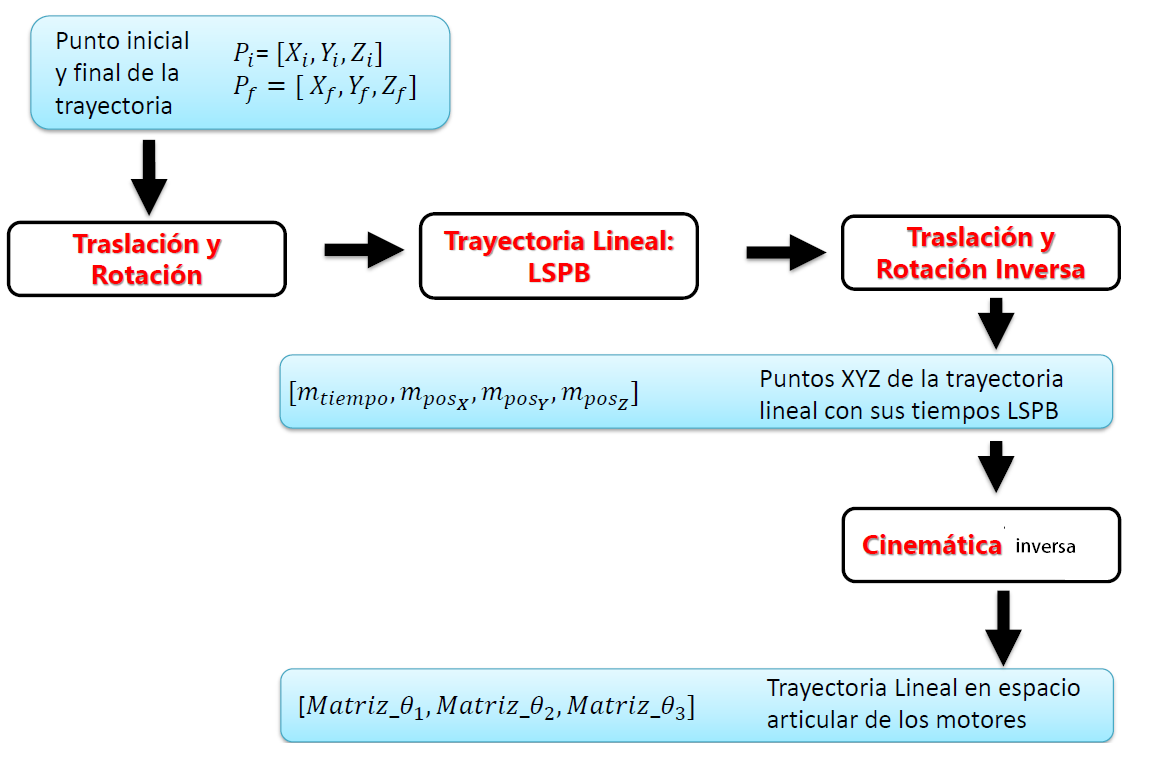
\includegraphics[width=1\linewidth]{Main/Chapter6/Images6/cap6_trayectory_4.png}
            \caption{Fotografía de un paraguas}
            \label{f:cap6_trayectory_4}
        \end{figure}
        
    A partir de de el punto inicial $P_i$ y el punto final $P_f$ se realiza una traslación y 2 rotaciones para aplicar la escala temporal de perfil trapezoidal y la interpolación del camino geométrico lineal. Luego se aplica traslación y rotaciones inversas para obtener la trayectoria en el espacio cartesiano respecto al sistema de referencia general.Finalmente se emplea la cinemática inversa para conseguir las trayectorias en el espacio articular de los actuadores.     
    
         \begin{figure}[htb]
            \centering
            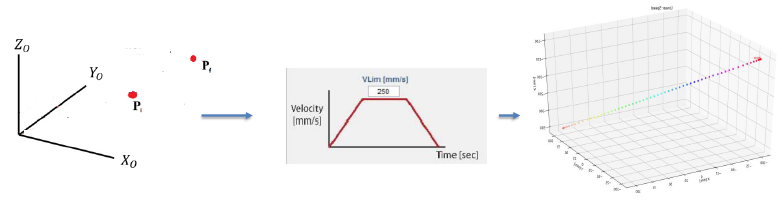
\includegraphics[width=0.9\linewidth]{Main/Chapter6/Images6/cap6_trayectory_1.png}
            \caption{Fotografía de un paraguas}
            \label{f:cap6_trayectory_5}
        \end{figure}    
    \newpage
    
    

    \begin{algorithm}[H]
            \caption{Trayectoria} 
            \SetKwInput{KwInput}{Input}                % Set the Input
            \SetKwInput{KwOutput}{Output}              % set the Output
            \SetKwInput{KwObjetivo}{Objetivo}                % Set the Input
            \SetKwInput{Kwfile}{Nombre archivo}                % Set the Input
            
            \DontPrintSemicolon
              \KwObjetivo {Escala de tiempo perfil de velocidad Trapezoidal LSPB e interpolación de camino geometrico lineal }
              \Kwfile{$linear.speed.f.adams$}
              \KwInput{$q_0,q_1,v_{max},a_{max},{n}_{\Delta Tramo1},{n}_{\Delta Tramo2}$}
              \KwOutput{$tiempo,{X}_{rot_{\theta_y}},{\dot{X}}_{rot_{\theta_y}},{\ddot{X}}_{rot_{\theta_y}}$}
              
                % Set Function Names
              \SetKwFunction{FSum}{$ls.v.a.total$}
              \SetKwFunction{FSub}{$ls.v.a.puntual$}
            
              \tcc{FUNCION PRINCIPAL}
              \SetKwProg{Fn}{}{:}{}
              \Fn{\FSum{$q_0,q_1,v_{max},a_{max},{n}_{\Delta Tramo1},{n}_{\Delta Tramo2}$}}{
              \tcc{Parametros de Curva LSPB}
                ${n}_{\Delta Tramo3}={n}_{\Delta Tramo1}$  \tcp*{División Tramo 3 = Tramo 1}
            	$\tau=v_{max}/a_{max}$ \tcp*{Tiempo total del tramo 1 y tramo 3}
            	$s=signo(q1-q0)$\;
            	$T=s\frac{(q_1-q_0)}{v_{max}}+\tau$ \tcp*{Tiempo total de la trayectoria}
            	$\Delta_{tramo1}=(\tau)/{n}_{\Delta Tramo1}$\;
            	$\Delta_{tramo2}=(T-2\tau)/{n}_{\Delta Tramo2}$\;
            	$\Delta_{tramo3}=\Delta_{tramo1}$\;
            	$n_{total}=\sum_{i=1}^{3} n_{\Delta Tramoi}+1$\tcp*{Total puntos de discretizacion}

                \tcc{Verificar si alcanza la ${v}_{max}$ para {v}_{max}  }
            	$T_f=2\sqrt{\frac{q_1-q_0}{a_{max}}}$ \tcp*{Tiempo total de la trayectoria para ${a}_{max}$}
            	${v}_{max.por.acel}={a}_{max}(T_f/2)$\;
            	
                \If{{v}_{max.por.acel}\leq{v}_{max}}{
                		${v}_{max}={v}_{max.por.acel}$\;
                		$\tau=T_f/2$\;
                		$T=T_f$\;
                		$\Delta_{tramo1}=(\tau)/n_{\Delta Tramo1}$\;
                		$\Delta_{tramo2}=0$\;
                		${n}_{\Delta Tramo2}=0$\;
                		$n_{total}=\sum_{i=1}^{3} n_{\Delta Tramoi}+1$\;
                       }
                \tcc{Calulcar Curva LSBP}
                \For{ $i$ $in$ $range[0, n_{total}]$}    
                { 
                    $tiempo_i=tiempo_i+\Delta_{tramoi}$ \tcp*{$\Delta_{tramoi}$ depende de $i$}
            		$X=ls.v.a.puntual(q_0,q_1,v_{max},a_{max},tiempo_i)$ \tcp*{LSPB}
            		\tcc{Resultados Posición,Velocidad,Aceleración de LSBP}
            		$ ({X}_{rot_{\theta_y}}[i],{\dot{X}}_{rot_{\theta_y}}[i],{\ddot{X}}_{rot_{\theta_y}}[i])=(X[0],X[1],X[2])$\;
            		$tiempo[i]=tiempo_i$\;
                }
               \KwRet $[tiempo,{X}_{rot_{\theta_y}},{\dot{X}}_{rot_{\theta_y}},{\ddot{X}}_{rot_{\theta_y}}]$
              }
    \end{algorithm}
    
    \clearpage   
        
\begin{algorithm}
      \ContinuedFloat
      \caption{Trayectoria (Continuacion...)}
      \tcc{SUBFUNCIONES}
      \SetKwProg{Fn}{}{:}{}
      \Fn{\FSub{$q_0,q_1,v_{max},a_{max},{tiempo}_{actual}$}}{
            	$\tau=v_{max}/a_{max}$\;
            	$s=signo(q_1-q_0)$\;
            	$T=s\frac{(q_1-q_0)}{v_{max}}+\tau$\;
        \tcc{Ecuaciones  LSPB (\ref{eq:cap6_tray_1})}
        \tcc{Tramo 1}
          \If{$(0 \leq {tiempo}_{actual}\leq \tau)$}
            {
        		$q_{actual}=q_0+s\frac{a_{max}}{2}{({tiempo}_{actual})}^2$\;
        		$v_{actual}=s{a}_{max}({tiempo}_{actual})$\;
        		$a_{actual}=s{a}_{max}$\;
        		$ \KwRet[q_{actual},v_{actual},a_{actual}]$\;
            }
        \tcc{Tramo 2}
            \ElseIf{$(\tau < {tiempo}_{actual}\leq T-\tau)$}
            {
        		$q_{actual}=q_0-(s\frac{{v_{max}}^2}{2{a}_{max}})+(s*{v}_{max}*{tiempo}_{actual})$\;
        		$v_{actual}=s*{v}_{max}$\;
        		$a_{actual}=0$\;
        		$ \KwRet[q_{actual},v_{actual},a_{actual}]$\;
            }
        \tcc{Tramo 3}
            \ElseIf{$(T-\tau<{tiempo}_{actual}\leq T)$}
            {
        		$q_{actual}=q_1+s\left(-\frac{a_{max}T^2}{2}+a_{max}T({tiempo}_{actual})-\frac{a_{max}}{2}{({tiempo}_{actual})}^2\right)$\;
        		$v_{actual}=s(a_{max}T-a_{max}{tiempo}_{actual})$\;
        		$a_{actual}=s(-a_{max})$\;
        		$\KwRet[q_{actual},v_{actual},a_{actual}]$\;
            }
      }
\end{algorithm}
    
        \newpage
    
    

    \newpage

\section{Interfaz de visualización Rviz}

    ANGULOS NO PONERLOS CODIGO ANGULOS SE COPIAN E LA TESIS TANTO
    
    MOSTRAR Y EXPLICAR CODIGO XML CON IMAGENES PADRRES E HIJOS 
    
    L1 L2 PARAMETROS DE CAP 5
    
    DIAGRAMA DE FLUJO COMO EL DE FUNCIONES DE SOFARE ROS 
    RVIZ TF POSICIONADOR RVIZ
    
    CODIFOS:1  ANGULOS INTERIORES 2 POSICIONADOR RVIZ TIEMPO REAL 3 XML URFD 4 CONEXION XML URFD CON TF CON RVIZ NOMBRE ELEMENTOS
    
    







    \newpage


\section{ADAMS}
